\scriptsize
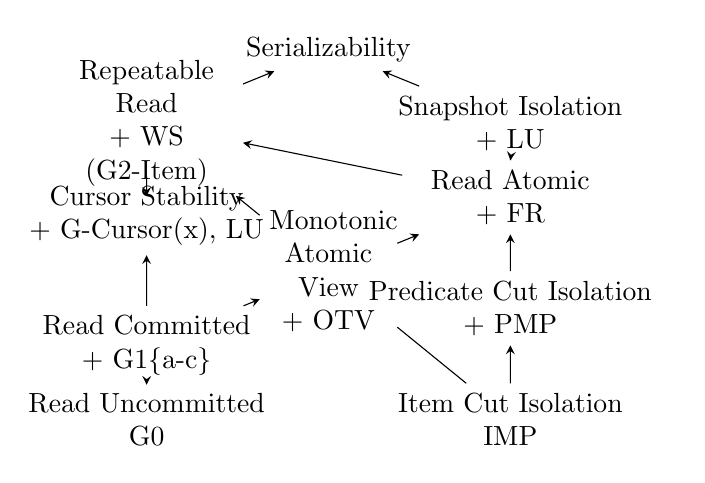
\begin{tikzpicture}[xscale=0.77,yscale=0.47,trim left=0.8cm]
%\draw[help lines] (0,0) grid (12,18);
\node[text width=4cm,align=center] (RU) at (3,1) {
\level{Read Uncommitted}  \\
\anomaly{G0}
};

\node[text width=4cm,align=center] (RC) at (3,3) {
\level{Read Committed}  \\
\anomaly{+ G1\{a-c\}}
};

\node[text width=4cm,align=center] (ICI) at (9,1) {
\level{Item Cut Isolation}  \\
\anomaly{IMP}
};

\node[text width=4cm,align=center] (PCI) at (9,4) {
\level{Predicate Cut Isolation}  \\
\anomaly{+ PMP}
};

\node[text width=1.5cm,align=center] (MAV) at (6,5) {
\level{Monotonic Atomic View}  \\
\anomaly{+ OTV}
};
% we place MAV below Adya’s PL-2L

\node[text width=4cm,align=center] (CS) at (3,6.5) {
\level{Cursor Stability}  \\
\anomaly{+ G-Cursor(x), LU}
};

\node[text width=2.5cm,align=center] (RA) at (9,7) {
\level{Read Atomic}  \\
\anomaly{+ FR}
};

\node[text width=3.3cm,align=center] (SI) at (9,9) {
\level{Snapshot Isolation}  \\
\anomaly{+ LU}
};

\node[text width=2.2cm,align=center] (RR) at (3,9) {
\level{Repeatable Read}  \\
\anomaly{+ WS (G2-Item)}
}; % Adya's

\node[text width=4cm,align=center] (S) at (6,11) {
  \level{Serializability}
};

\draw [->,>=stealth] (RU) -- (RC);
\draw [->,>=stealth] (ICI) -- (PCI);
\draw [->,>=stealth] (RC) -- (MAV);
% \draw [->,>=stealth,postaction={-,draw=white,dash pattern=on 0pt off 3cm on 3cm off 3cm}] (ICI) -- (RR);
\draw (ICI) -- (MAV);
\draw [->,>=stealth] (MAV) -- (RR);
\draw [->,>=stealth] (PCI) -- (RA);
\draw [->,>=stealth] (MAV) -- (RA);
\draw [->,>=stealth] (RA) -- (RR);
\draw [->,>=stealth] (RA) -- (SI);
\draw [->,>=stealth] (SI) -- (S);
\draw [->,>=stealth] (RR) -- (S);
\draw [->,>=stealth] (CS) -- (RR);
\draw [->,>=stealth] (RC) -- (CS);

\end{tikzpicture}
\caption{Hierarchy of isolation levels as described in~\cite{DBLP:journals/tods/BailisFGHS16}. All anomalies are covered except \anomaly{G-Cursor(x)}.}
\label{fig:isolation}
